\documentclass[10pt]{article}
\usepackage[margin=0.9in]{geometry}
\usepackage{amsmath,amssymb,amsthm,mathtools}
\usepackage{booktabs,multirow,makecell}
\usepackage{graphicx,subcaption}
\usepackage[dvipsnames]{xcolor}
\usepackage[colorlinks=true,linkcolor=MidnightBlue,citecolor=MidnightBlue,urlcolor=MidnightBlue]{hyperref}
\usepackage{enumitem}
\usepackage{microtype}
\setlist{nosep,leftmargin=1.3em}
\graphicspath{{../figures/}}

\newtheorem{proposition}{Proposition}
\newtheorem{corollary}{Corollary}
\theoremstyle{definition}
\newtheorem{definition}{Definition}
\theoremstyle{remark}
\newtheorem{remark}{Remark}

\newcommand{\E}{\mathbb{E}}
\newcommand{\R}{\mathbb{R}}
\newcommand{\pistop}{\pi_\phi}
\newcommand{\Lq}{\mathcal{L}_q}

\title{\textbf{Learned Stochastic Computation in Looped Transformers}\\[2pt]
\large When to stop, what to randomise, and how to spend a fixed compute budget}
\author{DA4022 Course Project}
\date{}

\begin{document}
\maketitle

\begin{abstract}
%ABSTRACT%
\end{abstract}

% =====================================================================
\section{Problem statement and summary}
\label{sec:intro}

The project brief asks to \emph{merge} two papers and to study the impact of
\emph{learned stochastic computation} under a \emph{fixed network size} and a
\emph{fixed average compute} budget:

\begin{itemize}
\item \textbf{Paper~1} (Kuo et al., \emph{Stabilizing Extrapolation in Looped Transformers via Learned Stochastic Stopping}, NeurIPS 2026)~\cite{kuo2026}.
A looped transformer applies one weight-tied block $K$ times.  Training it at a single, deterministic depth
makes length extrapolation brittle across runs; sampling the depth (``when to stop'') stabilises it, and
\emph{RL-Halting} learns the stopping distribution with REINFORCE.
\item \textbf{Paper~2} (von Oswald, Kobayashi, Akram, Steger, \emph{Learning Randomized Algorithms with Transformers}, ICLR 2025)~\cite{vonoswald2025}.
A transformer that receives a random seed as an extra input can learn a \emph{randomised algorithm}
(``what to compute'') when trained on a relaxed min--max objective
$\Lq=(\E_x[(\E_r \ell)^q])^{1/q}$; majority voting over seeds then amplifies its success probability.
\end{itemize}

Both papers inject randomness into neural computation, but along \emph{orthogonal axes}: paper~1 randomises the
\emph{amount} of computation (the halting time $\tau$), paper~2 randomises the \emph{path} of computation (a seed $r$).
Neither controls compute: paper~1's RL-Halting is trained without a cost on depth, and paper~2's fixed-depth
networks spend the same compute on every input.  We merge them into a single model, the
\textbf{stochastic looped transformer}, in which \emph{both} the halting time and the computation path are random
and learned, and study it at a fixed parameter count and an \emph{exactly enforced} average number of loop
iterations.

\paragraph{Contributions.}
\begin{enumerate}
\item \textbf{A unified model and objective} (\S\ref{sec:framework}): a looped transformer with a random-seed
  encoding re-injected at every iteration and a hazard-based stopping head, trained with the $q$-norm objective
  of paper~2 over seeds and the sampled-depth objective of paper~1, under an equality constraint
  $\E[\tau]=B$ on average compute.  The constraint is enforced with an augmented-Lagrangian dual (\emph{budgeted
  RL-Halting}), which removes the oscillations that plain dual ascent exhibits.
\item \textbf{Theory} (\S\ref{sec:theory}): (i) a matched-budget dominance result that makes comparisons
  between learned and hand-designed schedules fair; (ii) a \emph{Yao principle for stopping}: under ERM the
  optimal stopping policy at any budget is deterministic except on at most one input, so the stochasticity of
  RL-Halting can only act as a \emph{training-time regulariser}, while seed randomness can be a genuine
  \emph{inference-time mixed strategy}; (iii) a \emph{Jensen penalty}: stopping times that are random but
  independent of the realised computation lose accuracy at fixed mean compute when returns to depth are
  concave; (iv) a closed-form \emph{breadth-vs-depth} rule for spending a fixed total compute on $k$ seeds
  of $t$ loops each, $t^\star=\arg\max_t -\log(1-s(t))/t$.
\item \textbf{Experiments} (\S\ref{sec:seq}, \S\ref{sec:color}): length generalisation (Dyck-1 and Copy,
  paper~1's tasks) and distributed 3-colouring of cycles (paper~2's task, now looped so that one iteration is
  one communication round), with 9 schedules $\times$ 4--5 seeds and $\sim$150 colouring runs, all at a fixed
  parameter count and with compute accounted for at training and inference time.
\end{enumerate}

%FINDINGS%

% =====================================================================
\section{Background}
\label{sec:background}

\paragraph{Looped transformers and stopping schedules (paper~1).}
Let $E(x)\in\R^{m\times d}$ be token embeddings.  A looped transformer iterates
$H^{(t)}=\mathrm{Block}_\theta(H^{(t-1)}+E(x))$, $H^{(0)}=0$, and reads out logits from $H^{(K)}$.  A stopping
schedule $K\sim\pi(\cdot\mid x)$ determines the depth at which each training example is supervised:
fixed ($K=c$), length-matched ($K=n$), uniformly randomised ($K=n+\Delta$, $\Delta\sim\mathrm{U}\{-w,\dots,w\}$) or
learned (RL-Halting).  RL-Halting parameterises a hazard $\lambda_t=\sigma(q_\phi(\mathrm{Pool}(H^{(t)})))$,
$\pistop(\tau=t\mid x)=\lambda_t\prod_{i<t}(1-\lambda_i)$, samples $\tau$, supervises at depth $\tau$ only, and
updates $\phi$ with REINFORCE on the reward $-\ell(\theta;x,y,\tau)$ plus an entropy bonus.  Paper~1 finds that
stochastic schedules shrink run-to-run variance of out-of-distribution (OOD) accuracy and that RL-Halting
often improves the accuracy--stability trade-off, but can also stabilise a sub-optimal computation.

\paragraph{Learned randomised algorithms (paper~2).}
A model $A_\theta(x,r)$ receives a random seed $r$ (``random seed encoding'', concatenated to the tokens).
Under expected risk the seed is useless (Yao's principle: some deterministic seed is at least as good on
average), so ERM-trained models ignore it.  Under the relaxed min--max loss
$\Lq(\theta)=\E_x\big[(\E_r\,\ell(A_\theta(x,r)))^q\big]^{1/q}$, $q>1$, randomisation can be strictly better
(their Prop.~1): the model learns a distribution over deterministic algorithms so that no input is failed by
all of them, and majority voting (or, for verifiable outputs, best-of-$k$) amplifies the success probability.
Their tasks include associative recall, grid-world exploration, and distributed 3-colouring of cycles.

% =====================================================================
\section{A unified stochastic looped transformer}
\label{sec:framework}

\paragraph{Model.}
All models in this report share one architecture (Fig.~\ref{fig:model}):
\begin{equation}
H^{(t)}=\mathrm{LN}\Big(\mathrm{Block}_\theta\big(H^{(t-1)}+E(x)+W_r\,r_t\big)\Big),\quad
\text{logits}_t=W_o H^{(t)},\quad
\lambda_t=\sigma\big(w_\phi^\top \mathrm{Pool}(\mathrm{sg}[H^{(t)}])+b_\phi\big),
\label{eq:model}
\end{equation}
where $H^{(0)}=0$, the input $E(x)$ is re-injected at every iteration, and $r_t\in\R^{16}$
is a random seed encoding.  The seed can be absent ($r_t=0$), fixed ($r_t=r_0$; paper~2's $A_{r_0}$ baseline),
drawn once per example (or per vertex), or drawn afresh at every iteration (``loop'' / ``node-loop'' seeds,
which give a multi-round algorithm fresh random bits each round).  Every model owns $W_r$ and the stopping
head whether or not it uses them, so \textbf{all variants have exactly the same parameter count}.
$\mathrm{sg}$ is stop-gradient: the stopping head reads, but does not shape, the representation (as in paper~1).

\paragraph{Objective.}
With $\ell(\theta;x,y,r,\tau)$ the loss after $\tau$ iterations with seed stream $r$,
\begin{equation}
\min_{\theta,\phi}\;\Lq(\theta,\phi)=\Big(\E_x\big[\big(\E_{r}\,\E_{\tau\sim\pistop(\cdot\mid x,r)}\,\ell(\theta;x,y,r,\tau)\big)^q\big]\Big)^{1/q}
\quad\text{s.t.}\quad \E_x\E_r\E_{\tau\sim\pistop}[\tau]=B .
\label{eq:objective}
\end{equation}
Special cases recover both papers: no seed, $q=1$, $\pistop=\delta_n$ or $\mathrm{U}(n\pm w)$ gives paper~1's
deterministic and randomised schedules; learned $\pistop$ without constraint is RL-Halting; fixed depth with seeds
and $q>1$ is paper~2.  In practice each minibatch holds $b$ examples $\times$ $m$ seeds (total batch fixed, so
compute per step is unchanged by $m$), the inner expectation over $\tau$ is estimated with 4 samples from
$\pistop$, $\theta$ receives the ordinary gradient of the sampled-depth loss, and $\phi$ receives the REINFORCE
gradient $(R-b)\nabla_\phi\log\pistop(\tau)$ with $R=-\ell$, a moving-average baseline $b$, and an entropy bonus.

\paragraph{Budgeted RL-Halting (enforcing fixed average compute).}
The constraint in~\eqref{eq:objective} is an \emph{equality}: we want every method to use \emph{the same}
average compute, not merely at most $B$.  Because $D(\phi)=\E_x\sum_t t\,\pistop(t\mid x)$ is differentiable in
$\phi$, we add the augmented-Lagrangian term
\begin{equation}
\mathcal{P}(\phi)=\lambda\,(D-B)+\tfrac{\rho}{2}(D-B)^2,\qquad \lambda\leftarrow\lambda+\eta\,(D-B),
\label{eq:al}
\end{equation}
($\rho=1,\eta=5\cdot10^{-3}$).  With plain dual ascent ($\rho=0$) the multiplier integrates the error and the
average depth oscillated between 1.4 and 6.0 rounds around a budget of 4 in our pilot; with~\eqref{eq:al} it stays
within $\pm0.15$ of the budget for the whole run (Appendix~\ref{app:dual}).

\paragraph{Compute accounting.}
\emph{Training compute} is the average supervised depth (and, separately, the unrolled depth of the batch).
\emph{Inference compute} is the number of block applications per input: $K$ for fixed depth, $n$ for
length-matched rules, $\arg\max_t\pistop(t\mid x)$ for paper~1's policy (which requires unrolling to the test
horizon), and the realised $\tau$ for the \emph{on-line median rule} we add (stop at the first $t$ with
$\sum_{i\le t}\pistop(i)\ge\frac12$), which is computable while looping.  Running $k$ seeds multiplies compute by $k$.

\paragraph{Free amplification from the trajectory.}
A looped model produces a prediction at every depth, so the stopping distribution itself induces a distribution
over outputs.  The \emph{depth vote} returns its mode,
$\hat y=\arg\max_{y}\sum_t\pistop(t\mid x)\,\mathbb{1}[\hat y_t=y]$ --- paper~2's majority vote, but over the
randomness of \emph{when} to stop rather than over seeds, at no additional cost beyond the horizon already
unrolled by the arg-max policy.

\begin{figure}[t]
\centering
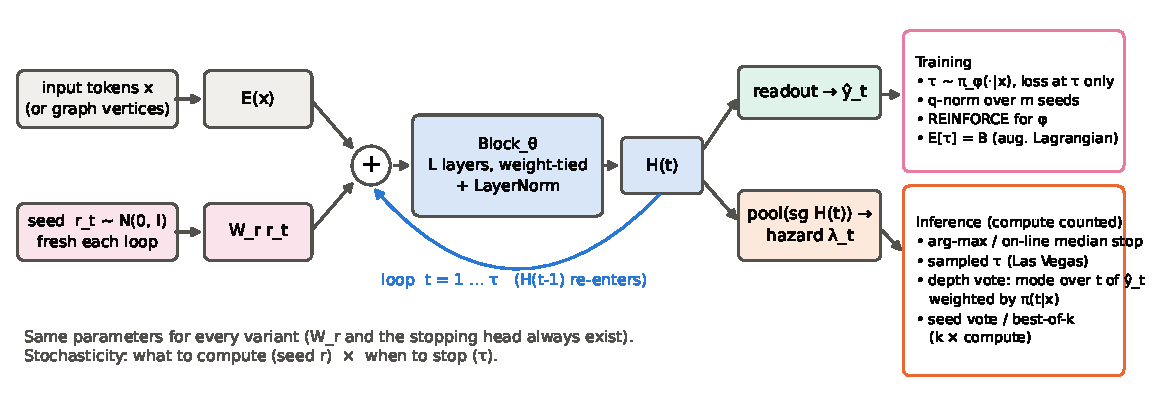
\includegraphics[width=0.92\linewidth]{model_diagram}
\caption{The stochastic looped transformer.  One weight-tied block (fixed parameters) is applied $\tau$ times.
A seed $r_t$ (paper~2) is projected and injected with the input at each iteration; a stopping head (paper~1)
emits a hazard $\lambda_t$ from the pooled, detached state.  Training samples $\tau\sim\pistop$, supervises only
at $\tau$, aggregates losses over seeds with the $q$-norm, and keeps $\E[\tau]=B$ with an augmented Lagrangian.}
\label{fig:model}
\end{figure}

% =====================================================================
\section{Theory: what stochastic computation can and cannot buy at fixed compute}
\label{sec:theory}

Throughout, $\ell(x,t)$ denotes the loss of a fixed network $\theta$ on input $x$ at depth $t$, and
$s_x(t)=\Pr_r[A_\theta(x;r,t)\text{ correct}]$ its success probability over seeds.

\begin{proposition}[Matched-budget dominance]\label{prop:dominance}
Let $\Pi_B=\{\pi:\E_x\E_{\tau\sim\pi(\cdot|x)}[\tau]=B\}$.  If a hand-designed schedule $\sigma$ lies in $\Pi_B$
---e.g.\ $\tau\equiv B$ for integer $B$, $\tau=n$ with $B=\E[n]$, or $\tau=n+\Delta$ with symmetric $\Delta$ and
no clipping--- then $\min_{\theta,\pi\in\Pi_B}\E\,\ell\le\min_\theta\E\,\ell(\theta,\sigma)$.
\end{proposition}
\begin{proof}$\sigma$ is feasible for the left-hand problem.\end{proof}
The statement is elementary, but it fixes the protocol: a learned schedule should be compared with hand-designed ones
\emph{inside} $\Pi_B$.  Unconstrained RL-Halting may buy its gains with extra depth; budgeted RL-Halting cannot.

\begin{proposition}[Yao's principle for stopping]\label{prop:yao}
Let $\mathcal X$ be finite with probabilities $p_x$ and depths $\{1,\dots,T\}$.  For fixed $\theta$, the problem
$\min_\pi\sum_x p_x\sum_t\pi(t|x)\ell(x,t)$ subject to $\sum_x p_x\sum_t\pi(t|x)\,t=B$ has an optimal solution in
which $\pi(\cdot|x)$ is a point mass for every input except at most one.  Without the budget constraint, a fully
deterministic policy $\tau^\star(x)=\arg\min_t\ell(x,t)$ is optimal.
\end{proposition}
\begin{proof}
The problem is a linear program in the $|\mathcal X|T$ variables $\pi(t|x)\ge0$ with $|\mathcal X|$ normalisation
equalities and one budget equality.  If it is feasible and bounded (it is: the feasible set is compact) it attains
its optimum at a basic feasible solution, which has at most $|\mathcal X|+1$ non-zero variables.  Each input needs
at least one non-zero variable, so at most one input has two.  Without the budget row there are $|\mathcal X|$
constraints and each $\pi(\cdot|x)$ is a point mass.
\end{proof}
\begin{remark}
Under the training objective of the stopping head, stochastic stopping is never needed at optimum; the entropy
of a learned stopping distribution is maintained only by the entropy bonus and by the non-stationarity of $\theta$
(paper~1 indeed reports collapse to a near-deterministic schedule without the entropy term).  Its benefit must
therefore come from \emph{how it shapes the training of $\theta$} (paper~1's gradient-averaging and
loop-consistency mechanisms), not from being a mixed strategy at inference.  Seed randomness is different:
under $\Lq$ with $q>1$, paper~2's Prop.~1 shows that mixtures over $\theta$-implemented algorithms can be strictly
optimal.  The two stochastic channels of the merged model thus play \emph{different} roles, which our
experiments confirm (\S\ref{sec:seq}, \S\ref{sec:color}).
\end{remark}

\begin{proposition}[Jensen penalty of uninformed stochastic stopping]\label{prop:jensen}
Fix $x$ and suppose $t\mapsto s_x(t)$ is concave on $\{1,\dots,T\}$ (diminishing returns to depth).  For every
stopping distribution $\pi$ that is independent of the seed stream (i.e.\ of the realised computation) and has
integer mean $\E_\pi[\tau]=b$, the success at random depth satisfies $\E_{\tau\sim\pi}[s_x(\tau)]\le s_x(b)$.
\end{proposition}
\begin{proof}
Extend $s_x$ to the piecewise-linear interpolation $\bar s_x$ on $[1,T]$, which is concave because the discrete
increments are non-increasing.  By independence, $\Pr[\text{correct}]=\E_\tau[s_x(\tau)]=\E_\tau[\bar s_x(\tau)]\le
\bar s_x(\E\tau)=s_x(b)$ by Jensen's inequality.
\end{proof}
Random stopping can beat fixed depth at equal mean compute only if it is \emph{informed}: either it varies across
inputs (allocating depth to hard inputs) or it depends on the realised trajectory (stopping when done).  The
latter is exactly the Monte Carlo $\to$ Las Vegas conversion of randomised-algorithm theory: a Las Vegas algorithm
has a random run time and stops when its output is verified.

\begin{proposition}[Breadth vs depth at fixed total compute]\label{prop:breadth}
Suppose $k$ runs with independent seeds, each of depth $t$, are combined by a verifier (success if any run is
correct), and let $g_x(t)=-\log(1-s_x(t))$.  At total compute $C=kt$,
\[
S_x(k,t)=1-(1-s_x(t))^k=1-\exp\!\big(-C\,g_x(t)/t\big),
\]
so the compute-optimal depth is $t^\star_x=\arg\max_t g_x(t)/t$ and the optimal breadth is $k=C/t^\star_x$.
Moreover (a) if the model is deterministic ($s_x(t)\in\{0,1\}$) then $S_x(k,t)=s_x(t)$ for all $k$: breadth is
worthless and every input failed at depth $t$ is failed by every allocation of breadth; (b) if
$\min_x s_x(t)\ge\varepsilon>0$, the worst-case success is at least $1-e^{-k\varepsilon}$.
\end{proposition}
\begin{proof}Independence gives the first identity; the rest is monotonicity of $1-e^{-u}$ and $1-\varepsilon\le e^{-\varepsilon}$.\end{proof}
For a ``memoryless'' algorithm, $s(t)=1-e^{-\alpha t}$, the ratio $g/t=\alpha$ is constant and allocation is
irrelevant; when returns to depth saturate, short runs and many seeds win; when there is a depth threshold below
which nothing works, depth must first reach the threshold.  We test this prediction in \S\ref{sec:color}.

% =====================================================================
%SETUP%
%RESULTS%

\clearpage
\begin{thebibliography}{99}\small
\bibitem{kuo2026} H.-Y. Kuo, E. M. Chayti, P. Reizinger, W. Brendel, M. Jaggi. Stabilizing Extrapolation in Looped Transformers via Learned Stochastic Stopping. \emph{NeurIPS}, 2026.
\bibitem{vonoswald2025} J. von Oswald, S. Kobayashi, Y. Akram, A. Steger. Learning Randomized Algorithms with Transformers. \emph{ICLR}, 2025.
\bibitem{fan2024} Y. Fan, Y. Du, K. Ramchandran, K. Lee. Looped Transformers for Length Generalization. \emph{ICLR}, 2025.
\bibitem{dehghani2018} M. Dehghani, S. Gouws, O. Vinyals, J. Uszkoreit, \L{}. Kaiser. Universal Transformers. \emph{ICLR}, 2019.
\bibitem{graves2016} A. Graves. Adaptive Computation Time for Recurrent Neural Networks. arXiv:1603.08983, 2016.
\bibitem{banino2021} A. Banino, J. Balaguer, C. Blundell. PonderNet: Learning to Ponder. arXiv:2107.05407, 2021.
\bibitem{williams1992} R. J. Williams. Simple statistical gradient-following algorithms for connectionist reinforcement learning. \emph{Machine Learning}, 8:229--256, 1992.
\bibitem{yao1977} A. C.-C. Yao. Probabilistic computations: toward a unified measure of complexity. \emph{FOCS}, 1977.
\bibitem{rice2021} L. Rice, A. Bair, H. Zhang, J. Z. Kolter. Robustness between the worst and average case. \emph{NeurIPS}, 2021.
\bibitem{angluin1980} D. Angluin. Local and global properties in networks of processors. \emph{STOC}, 1980.
\bibitem{linial1992} N. Linial. Locality in distributed graph algorithms. \emph{SIAM J. Computing}, 21(1):193--201, 1992.
\bibitem{cole1986} R. Cole, U. Vishkin. Deterministic coin tossing with applications to optimal parallel list ranking. \emph{Information and Control}, 70(1):32--53, 1986.
\bibitem{motwani1995} R. Motwani, P. Raghavan. \emph{Randomized Algorithms}. Cambridge University Press, 1995.
\bibitem{bertsekas1982} D. P. Bertsekas. \emph{Constrained Optimization and Lagrange Multiplier Methods}. Academic Press, 1982.
\bibitem{huang2016} G. Huang, Y. Sun, Z. Liu, D. Sedra, K. Weinberger. Deep Networks with Stochastic Depth. \emph{ECCV}, 2016.
\bibitem{schwarzschild2021} A. Schwarzschild et al. Can You Learn an Algorithm? Generalizing from Easy to Hard Problems with Recurrent Networks. \emph{NeurIPS}, 2021.
\bibitem{bansal2022} A. Bansal et al. End-to-end Algorithm Synthesis with Recurrent Networks: Logical Extrapolation Without Overthinking. \emph{NeurIPS}, 2022.
\bibitem{geiping2025} J. Geiping et al. Scaling up Test-Time Compute with Latent Reasoning: A Recurrent Depth Approach. arXiv:2502.05171, 2025.
\bibitem{wang2023} X. Wang et al. Self-Consistency Improves Chain of Thought Reasoning in Language Models. \emph{ICLR}, 2023.
\bibitem{zhou2024} Y. Zhou et al. Transformers Can Achieve Length Generalization But Not Robustly. arXiv:2402.09371, 2024.
\end{thebibliography}

%APPENDIX%
\end{document}
